e\section{Coil and yoke studies}
%\writer{Karsten Buesser, Uwe Schneekloth}{3}

A conceptual design of the ILD solenoid, the yoke and the cryostat had been developed for the ILD DBD, c.f.~\cite{ild:bib:Magnet_Note, ild:bib:Cryostat_Note}. Recently, studies have been done to optimise the engineering design of the magnet, to study the magnetic properties of the large and small ILD detector models, and to explore possible cost reductions.

\subsection{Magnet Engineering Studies}
A common study by KEK, Toshiba and Hitachi has been started toebeteer understand the engineering challenges in the design and manufacturing of the ILD solenoid coil and the Anti-DID. Figure~\ref{ILD:fig:solenoid_manufacturing} shows a conceptual design of the manufacturing process. While the three solenoid modules and the Anti-DID coils would be fabricated in industry, transportation boundary conditions require the assembly of the complete magnet on or close to the final detector site.
\begin{figure}[h!]
    \centering
    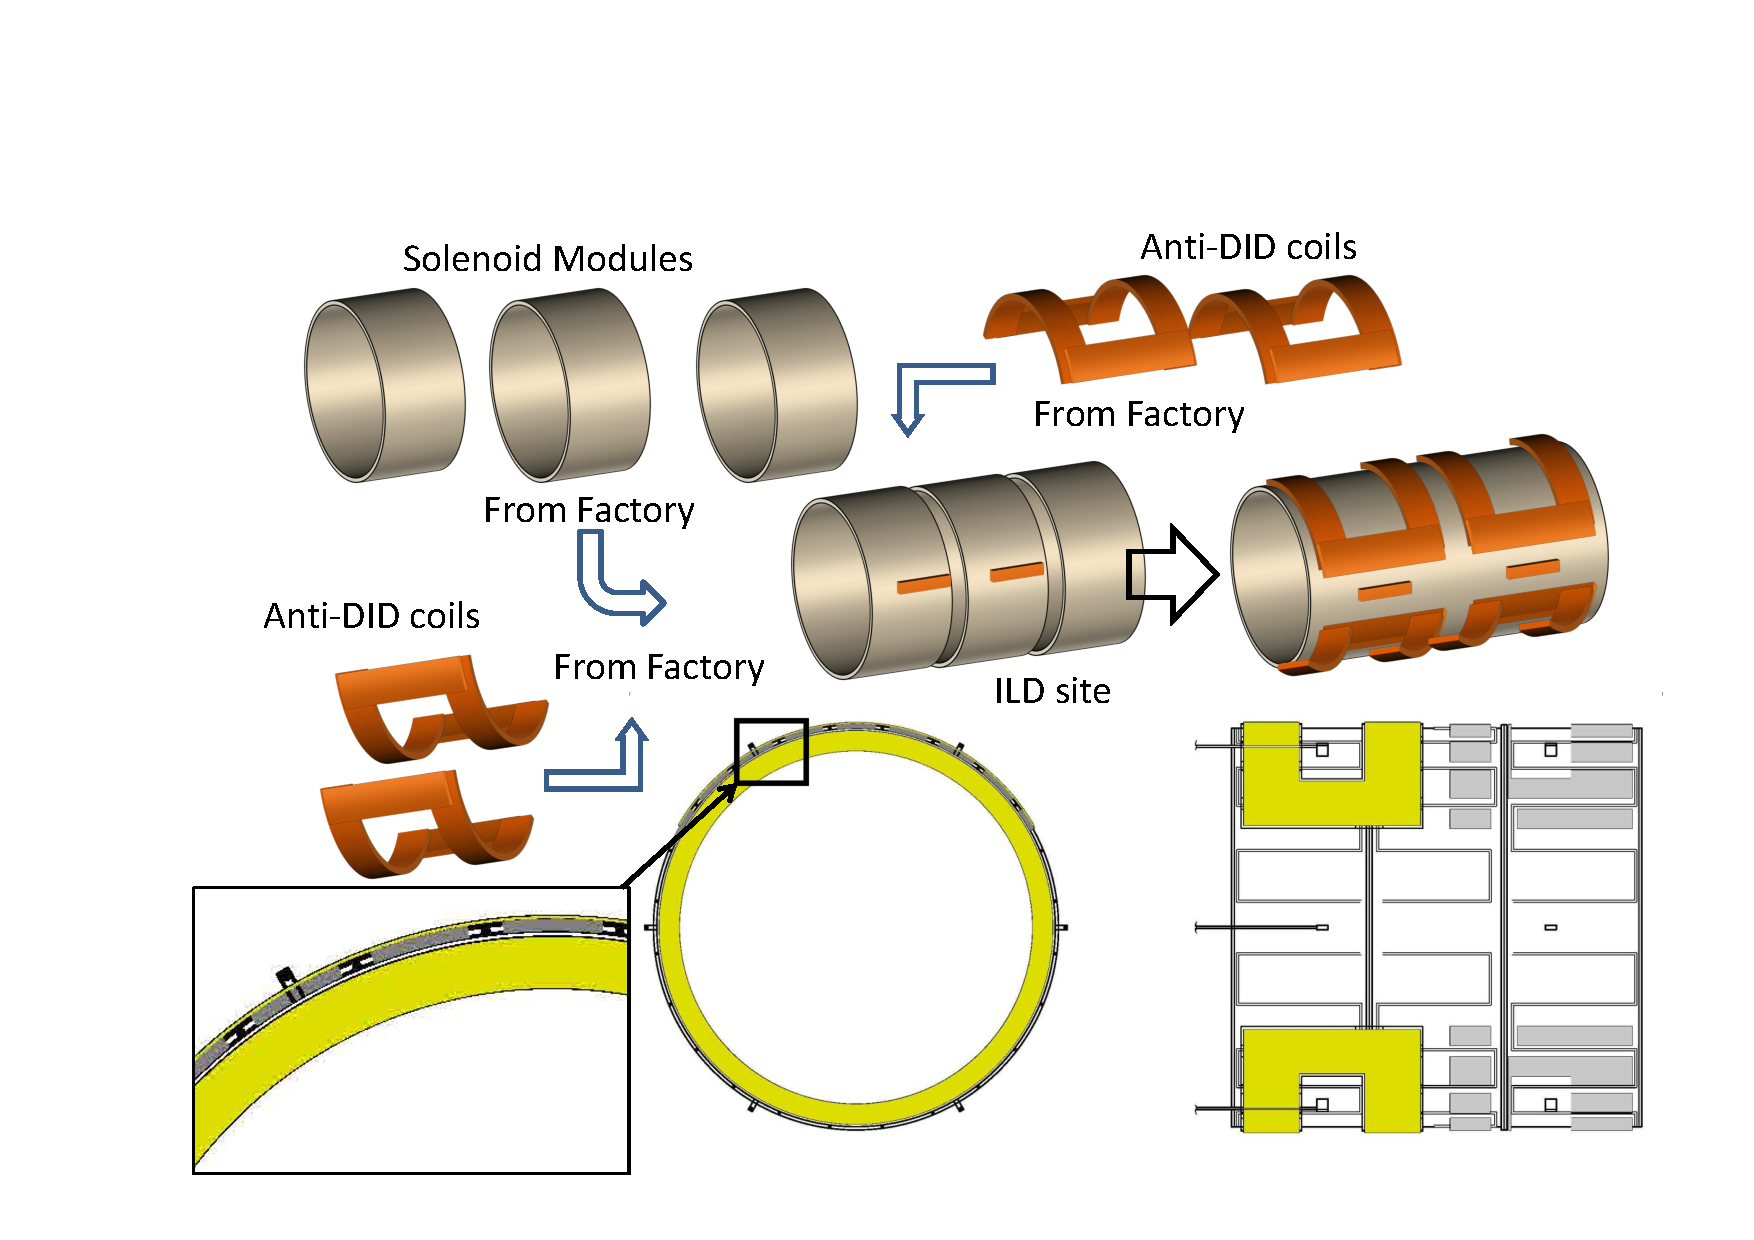
\includegraphics[width=0.8\hsize]{Integration/fig/Solenoid_Manufacturing.pdf}
    \caption{Conceptual manufacturing process of the ILD solenoid and the Anti-DID coils~\cite{ild:bib:Solenoid_Manufacturing}.}
    \label{ILD:fig:solenoid_manufacturing}
\end{figure}
A case study by Toshiba concluded that the main solenoid modules can be transported on street with the use of a specialised Jumbo Carrier while the modules of the Anti-DID would fit on a flatbed trailer~(figure~\ref{ILD:fig:magnet_transport}).
\begin{figure}[h!]
    \centering
    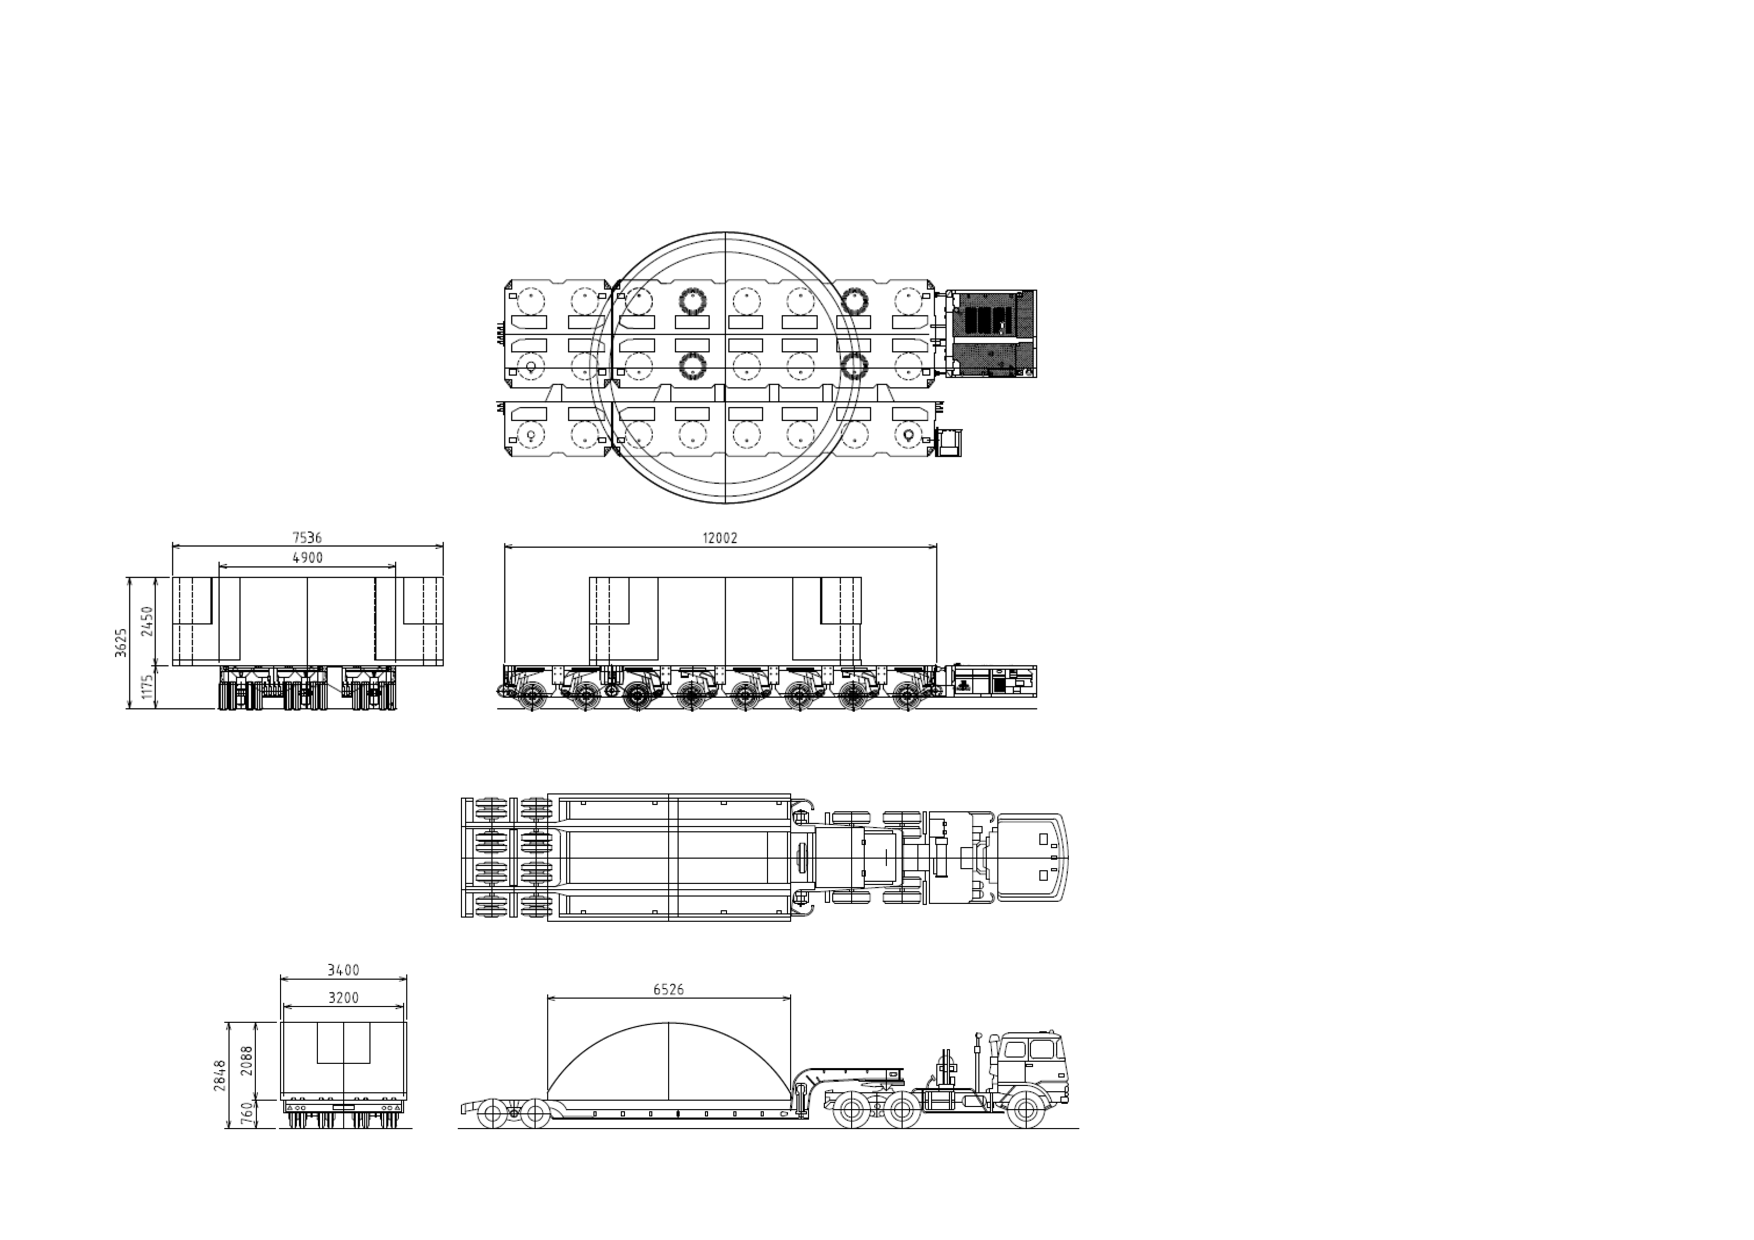
\includegraphics[width=0.8\hsize]{Integration/fig/Magnet_Transport.pdf}
    \caption{While a solenoid module requires transportation by a specialised Jumbo Carrier (top), the Anti-DID modules would fit on a low flatbed trailer (bottom)~\cite{ild:bib:Solenoid_Manufacturing}}
    \label{ILD:fig:magnet_transport}
\end{figure}

The so-called "Anti-DID" coil has been proposed to add a small additional dipole field to the solenoid for better suppression of backgrounds~(c.f. section~\ref{ild:sec:beam_backgrounds} and \cite{ild:bib:anti-did}). Figure~\ref{ILD:fig:anti_did_design} shows a conceptual design of the Anti-DID coils and the resulting simulated dipole field with a maximum value of 0.036~T. Splitting the Anti-DID coils in four makes construction at the manufacturer and transport to the ILC site easier (c.f.~figure~\ref{ILD:fig:magnet_transport}).

\begin{figure}[h!]
%\begin{center}
\begin{subfigure}{0.49\hsize} 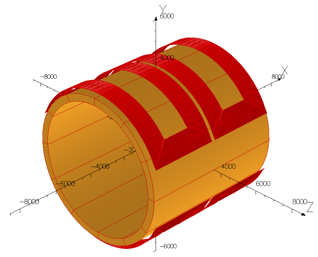
\includegraphics[width=\textwidth]{Integration/fig/Anti-DID.png}
\caption{ \label{ild:fig:anti_did_mechanics}}
 \end{subfigure}
%\hspace{0.03\textwidth}
\begin{subfigure}{0.49\hsize} 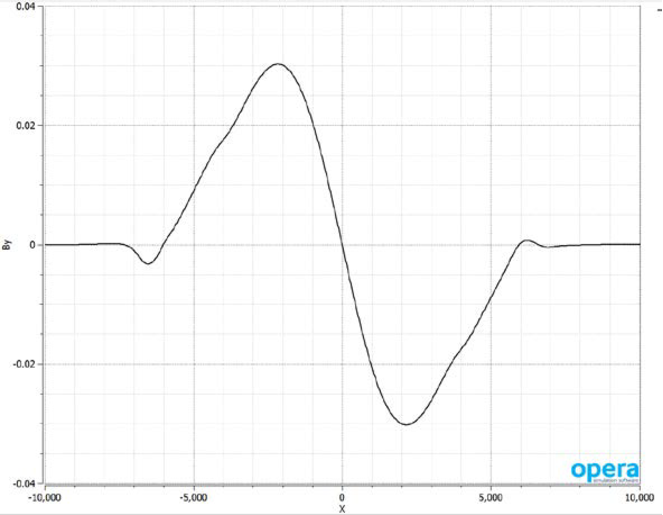
\includegraphics[width=\textwidth]{Integration/fig/Anti-DID_Field.pdf}
\caption{  \label{ild:fig:anti-did-field}}
 \end{subfigure}
%\end{center}
\caption{Conceptual design study of the Anti-DID coils (a) and simulated Anti-DID field (b)~\cite{ild:bib:anti-did-design}}
\label{ILD:fig:anti_did_design}
\end{figure}

\subsection{Field Optimisation Studies}

The coil and yoke system should provide at the same time a high magnetic field in the central region and low stray field on the outside of the detector. The nominal fields for the large (small) ILD detector model are 3.5T (4T). To allow for safety margins and possible extensions to higher field values, the coil design has been developed to reach 0.5T more in each case. Figure~\ref{ILD:fig:magnet_nominal} therefore shows the field map and the field distribution for the large ILD detector model and a maximum field of 4T. The corresponding distributions for the small ILD detector model are shown in figure~\ref{ILD:fig:magnet_small}. The field maps are the result of 3D magnetic field simulations. They are implemented in the simulation tools of the detector (chapter 7) to allow for reconstruction with maximum realism when this is required by specific studies such as beam background effects (section 6.5). 

\begin{figure}[t]
\begin{center}
\begin{subfigure}{0.9\hsize} 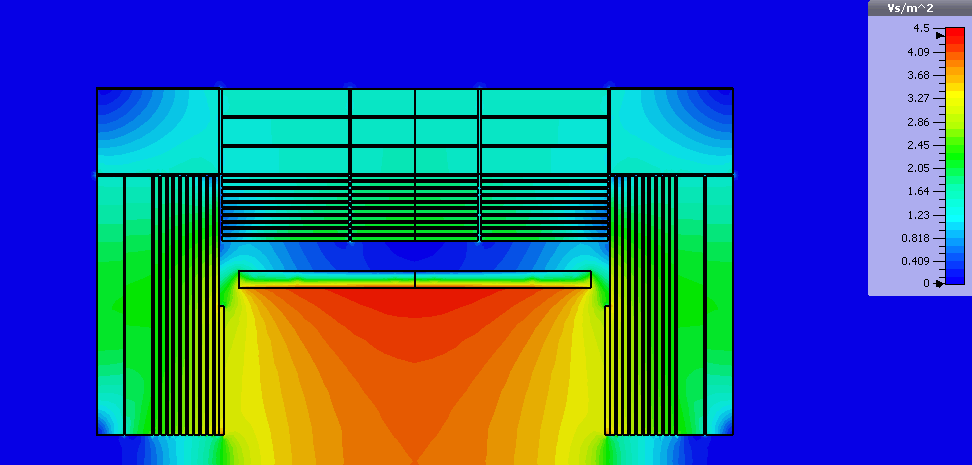
\includegraphics[width=\textwidth]{Integration/fig/field_nominal_4.png}
\caption{ \label{ild:fig:magnet_nominal_map}}
 \end{subfigure}
\hspace{0.03\textwidth}
\begin{subfigure}{0.9\hsize} 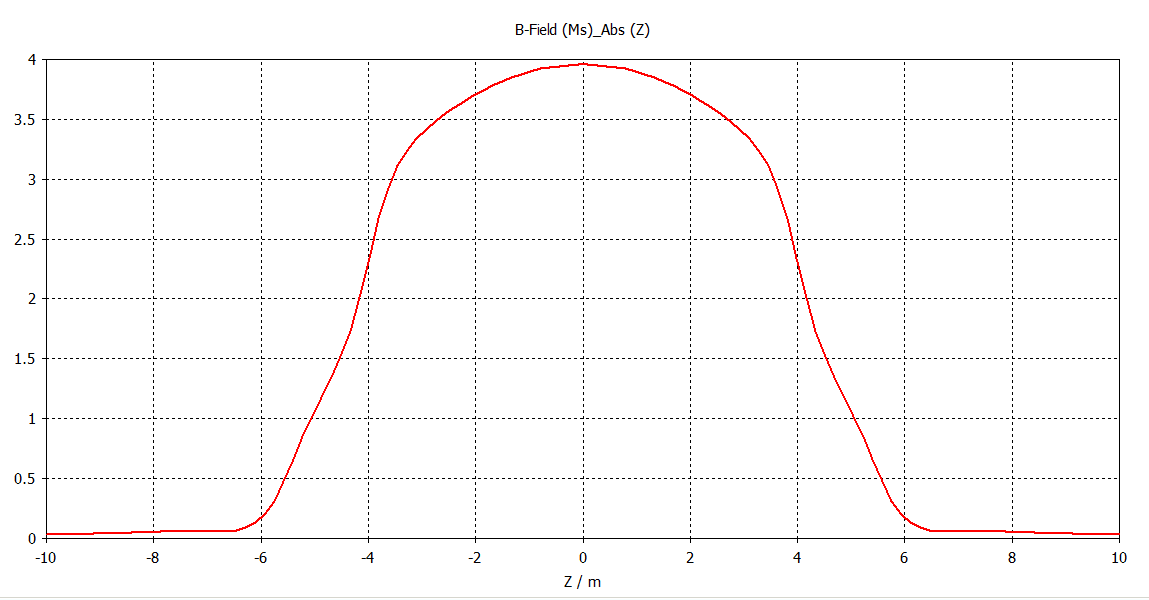
\includegraphics[width=\textwidth]{Integration/fig/field_nominal_4_plot.png}
\caption{  \label{ild:fig:magnet_nominal_field}}
 \end{subfigure}
\end{center}
\caption{Field map of the ILD solenoid for the large ILD model with a maximum field of 4~T (a) and field distribution along the detector axis (b)~\cite{ild:bib:Magnet_Simulations}}
\label{ILD:fig:magnet_nominal}
\end{figure}

\begin{figure}[t]
\begin{center}
\begin{subfigure}{0.9\hsize} 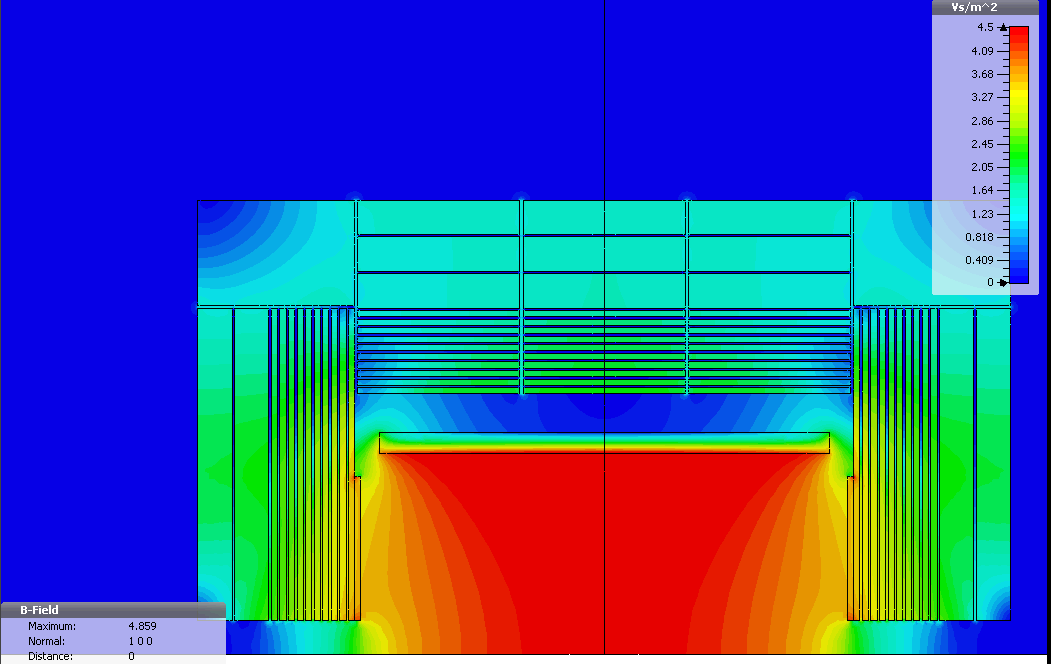
\includegraphics[width=\textwidth]{Integration/fig/field_small_4_5.png}
\caption{ \label{ild:fig:magnet_small_map}}
 \end{subfigure}
\hspace{0.03\textwidth}
\begin{subfigure}{0.9\hsize} 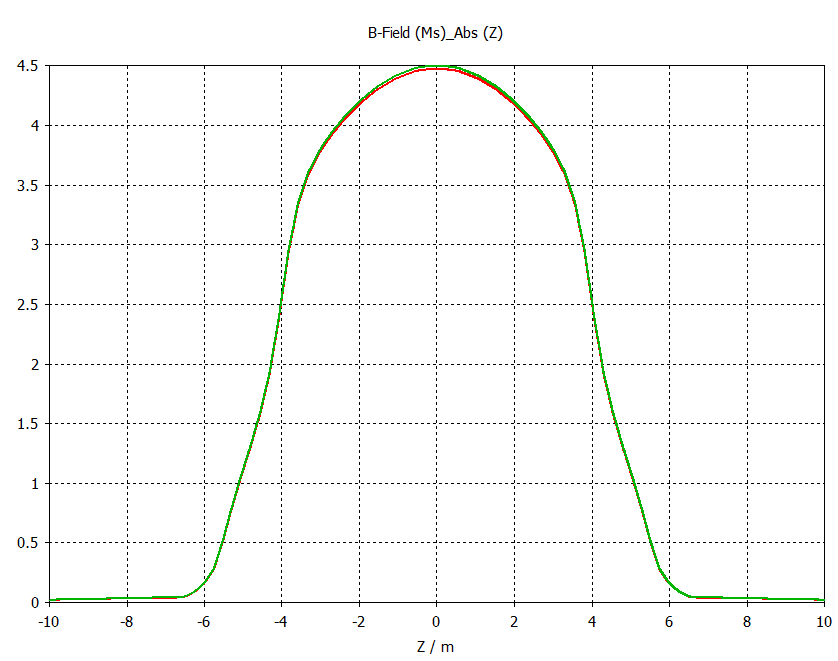
\includegraphics[width=\textwidth, height = 6cm]{Integration/fig/field_small_4_5_plot.png}
\caption{  \label{ild:fig:magnet_small_field}}
 \end{subfigure}
\end{center}
\caption{Field map of the ILD solenoid for the small ILD model with a maximum field of 4.5~T (a) and field distribution along the detector axis (b)~\cite{ild:bib:Magnet_Simulations}}
\label{ILD:fig:magnet_small}
\end{figure}


The ILD detector is expected to share its experimental environment with another detector, e.g. SiD, in a push-pull scenario. This model of operations assumes that each detector can run its magnetic field while still allowing the other detector crew to work on their detector with the use of standard iron-based tools. Therefore a limit on the maximum magnetic stray fields has been agreed upon at a maximum of 5~mT at a distance of 15~m from the detector axis~\cite{Parker:2009zz}. This requirement is the main driver for the thickness of the iron yoke of ILD. Figures~\ref{ILD:fig:magnet_nominal_stray} and \ref{ILD:fig:magnet_small_stray} show the simulated stray fields for the large and the small detector model at 4~T and 4.5~T maximum central field.
\begin{figure}[t]
\begin{center}
\begin{subfigure}{0.9\hsize} 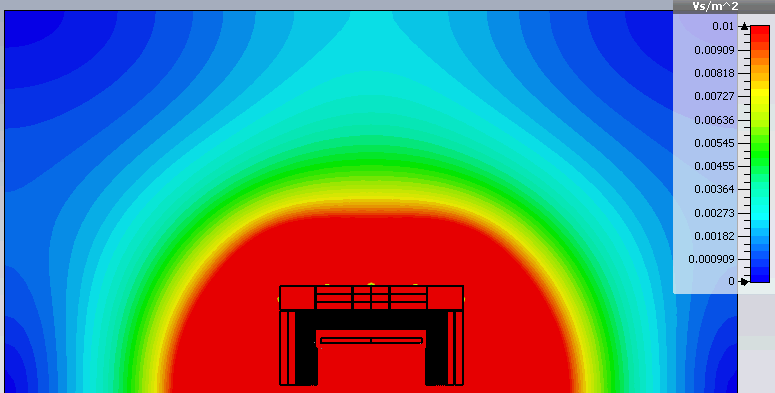
\includegraphics[width=\textwidth]{Integration/fig/strayfield_nominal_4.png}
\caption{ \label{ild:fig:magnet_nominal_stray_map}}
 \end{subfigure}
\hspace{0.03\textwidth}
\begin{subfigure}{0.9\hsize} 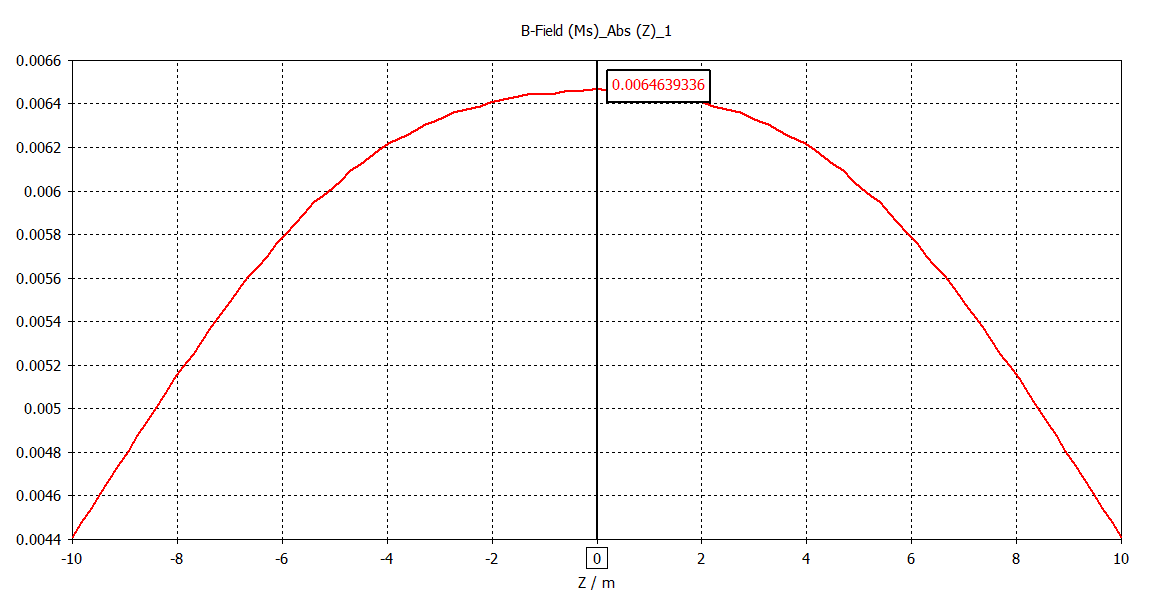
\includegraphics[width=\textwidth]{Integration/fig/strayfield_nominal_4_plot.png}
\caption{  \label{ild:fig:magnet_nominal_stray_field}}
 \end{subfigure}
\end{center}
\caption{Map of the ILD solenoid strayfield for the large ILD model with a maximum central field of 4~T (a) and field distribution at a distance of 15~m parallel to the detector axis (b)~\cite{ild:bib:Magnet_Simulations}.}
\label{ILD:fig:magnet_nominal_stray}
\end{figure}

\begin{figure}[h!]
\begin{center}
\begin{subfigure}{0.9\hsize} 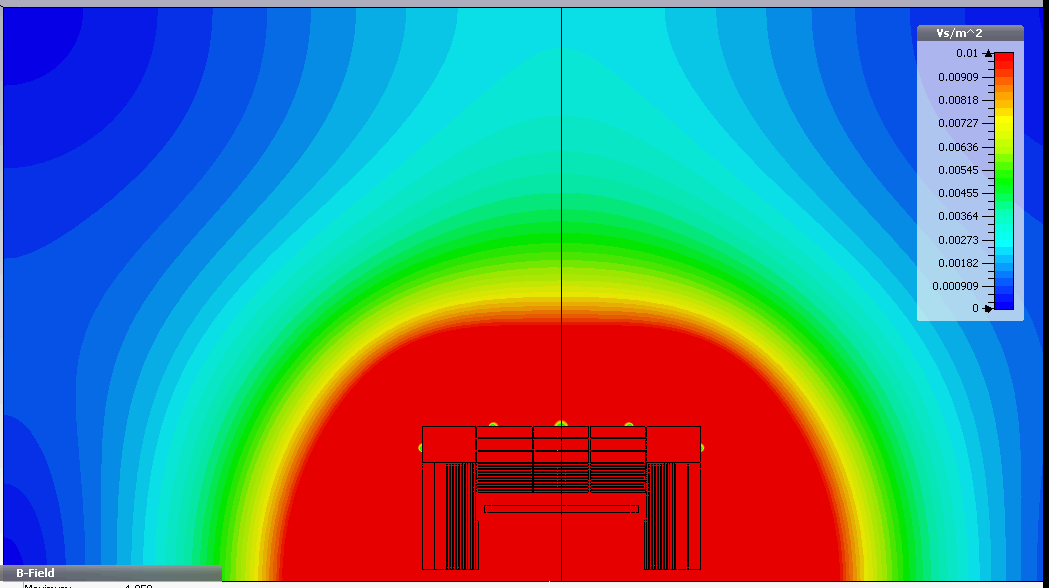
\includegraphics[width=\textwidth]{Integration/fig/strayfield_small_4_5.png}
\caption{ \label{ild:fig:magnet_small_stray_map}}
 \end{subfigure}
\hspace{0.03\textwidth}
\begin{subfigure}{0.9\hsize} 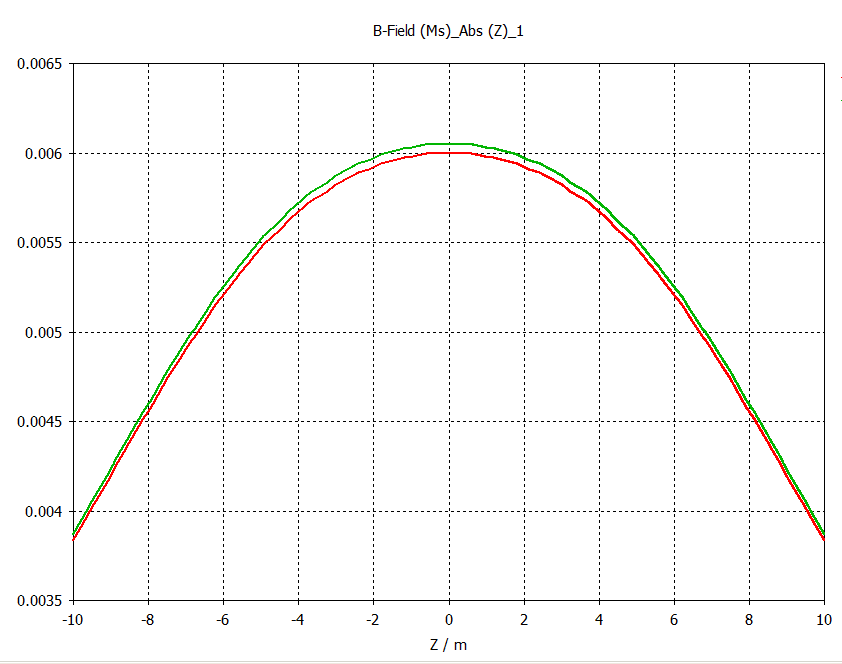
\includegraphics[width=\textwidth, height =6cm]{Integration/fig/strayfield_small_4_5_plot.png}
\caption{  \label{ild:fig:magnet_small_stray_field}}
 \end{subfigure}
\end{center}
\caption{Field map of the ILD solenoid for the small ILD model with a maximum field of 4.5~T (top) and field distribution at a distance of 15~m parallel to the detector axis (bottom)~\cite{ild:bib:Magnet_Simulations}.}
\label{ILD:fig:magnet_small_stray}
\end{figure}

Simulations have been done with different codes and the results are very consistent with an average value for the large detector of 5.6$\pm$0.6~mT for the maximum stray field at 15~m~\cite{ild:bib:Magnet_Simulations}. The stray fields for the small detector model are very similar. 

The stringent limits on the stray fields are a cost driver for ILC as they drive the thickness of the iron return yoke. If the thickness would be reduced by 60~cm, the maximum stray fields at 15~m would increase to 9.3$\pm$0.8~mT but at the same time reduce the cost for the yoke by about 20\% for the large ILD detector model~\cite{ild:bib:Magnet_Simulations}.

A cost reduction of in total $\approx$50\% can be reached if the iron yoke is reduced further to a thickness of 2.04~m (including gaps). The stray fields at 1~m distance from the outside of the yoke would be at the level of 100~mT which is acceptable for the operation of magnetically sensitive equipment and which is well below limits given by human safety regulations. The far stray fields in direction of the other detector need to be shielded in that case, e.g. by using a magnetic shielding wall. Figure~\ref{ILD:fig:magnet_wall} shows the simulation of the large ILD detector model magnetic fields with a reduced yoke and a shielding wall.

Though this concept looks attractive, further studies are required. The shielding wall needs to be mobile and has to follow the push-pull movements. An engineering solution needs to be developed. Another problem is the radiation shielding. In the present design, the thick iron yoke serves as a radiation shield and allows for access to the outer side of the detector while the ILC delivers beams to the interaction region~\cite{ild:bib:Radiation_Hall}. A reduced yoke might be too thin to serve for this purpose alone and additional radiation shielding, e.g. made from concrete, might need to be added. 
\begin{figure}[htb]
    \centering
    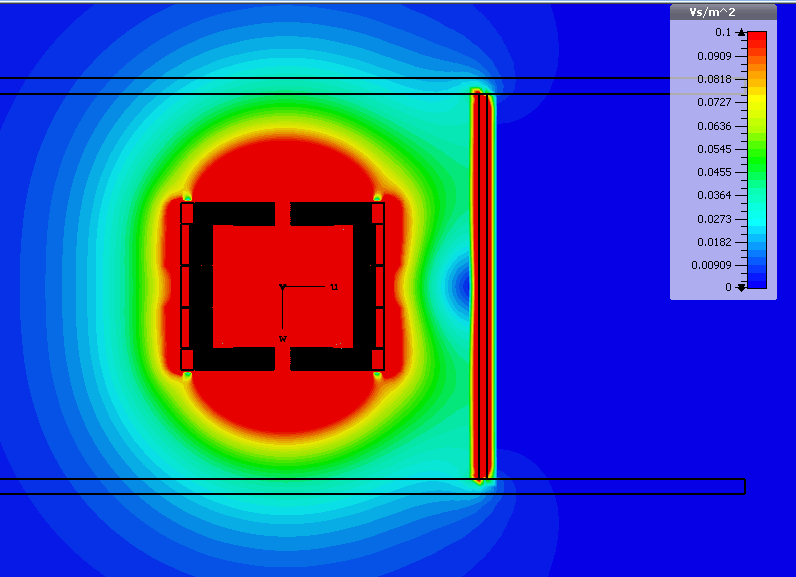
\includegraphics[width=0.8\hsize]{Integration/fig/magnet_wall.png}
    \caption{Field map of the ILD solenoid for the large ILD model with a iron shielding wall towards the direction of the other detector in the experimental hall~\cite{ild:bib:Magnet_Simulations}.}
    \label{ILD:fig:magnet_wall}
\end{figure}


